\documentclass{standalone}
\usepackage{tikz}
\usetikzlibrary{patterns, positioning}
\usetikzlibrary{shapes.misc}
\usepackage[outline]{contour}
\contourlength{1.5pt} 


\begin{document}
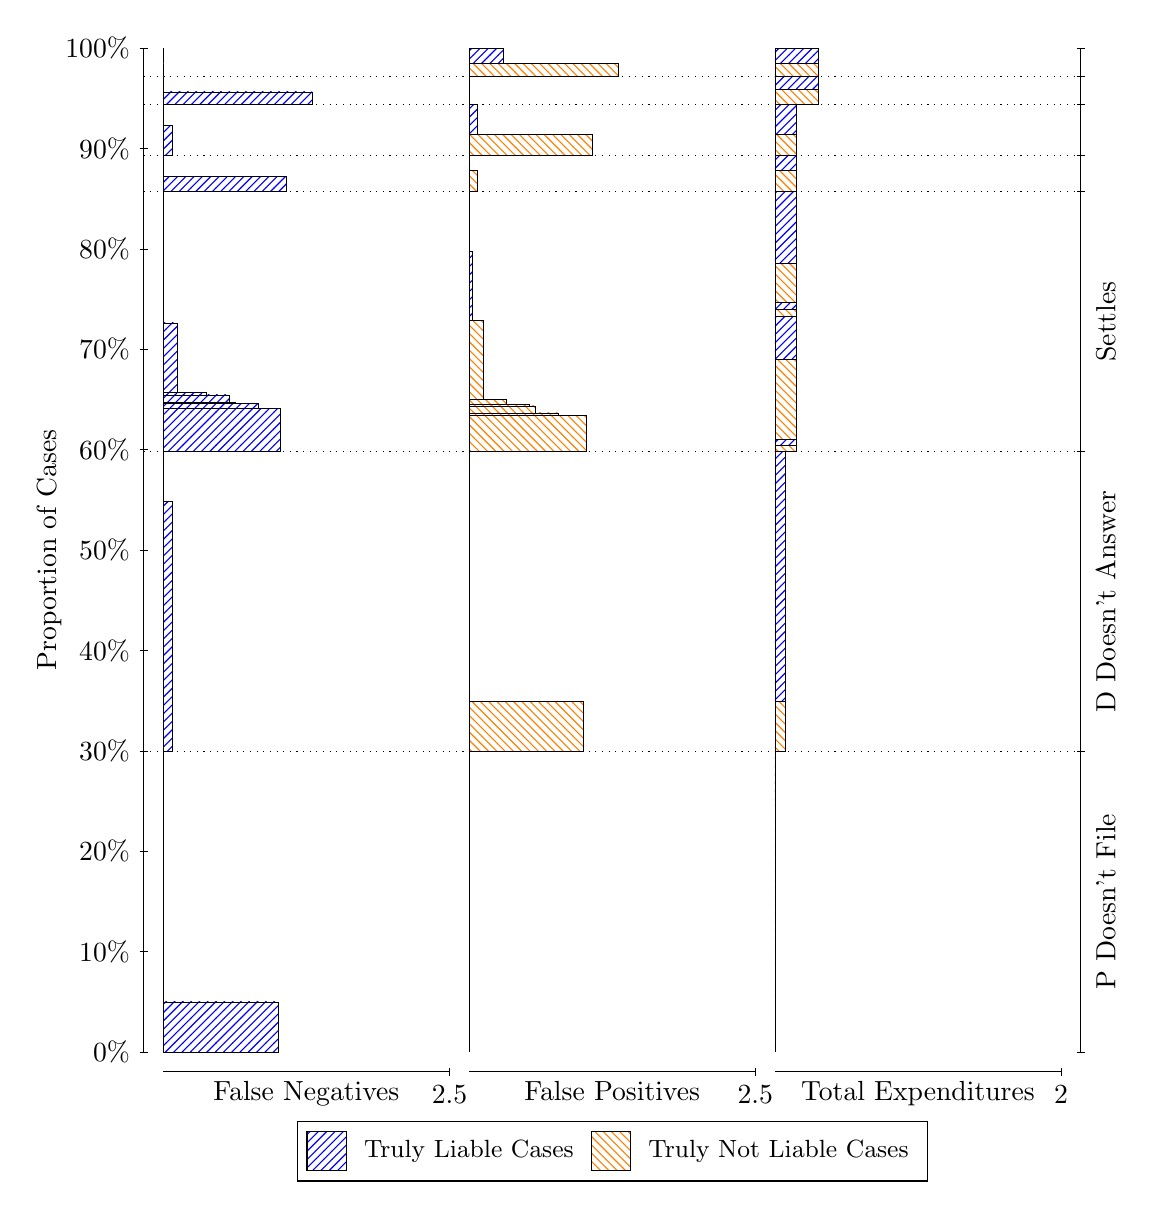
\begin{tikzpicture}
\draw[black, very thin] (1.5,1.75) -- (1.5,14.5);
\node[rotate=90, text=black, anchor=center] at (0.3, 8.125) {Proportion of Cases};
\draw[black, very thin] (1.45,1.75) -- (1.55,1.75);
\node[text=black, anchor=east] at (1.45, 1.75) {0\%};
\draw[black, very thin] (1.45,3.025) -- (1.55,3.025);
\node[text=black, anchor=east] at (1.45, 3.025) {10\%};
\draw[black, very thin] (1.45,4.3) -- (1.55,4.3);
\node[text=black, anchor=east] at (1.45, 4.3) {20\%};
\draw[black, very thin] (1.45,5.575) -- (1.55,5.575);
\node[text=black, anchor=east] at (1.45, 5.575) {30\%};
\draw[black, very thin] (1.45,6.85) -- (1.55,6.85);
\node[text=black, anchor=east] at (1.45, 6.85) {40\%};
\draw[black, very thin] (1.45,8.125) -- (1.55,8.125);
\node[text=black, anchor=east] at (1.45, 8.125) {50\%};
\draw[black, very thin] (1.45,9.4) -- (1.55,9.4);
\node[text=black, anchor=east] at (1.45, 9.4) {60\%};
\draw[black, very thin] (1.45,10.675) -- (1.55,10.675);
\node[text=black, anchor=east] at (1.45, 10.675) {70\%};
\draw[black, very thin] (1.45,11.95) -- (1.55,11.95);
\node[text=black, anchor=east] at (1.45, 11.95) {80\%};
\draw[black, very thin] (1.45,13.225) -- (1.55,13.225);
\node[text=black, anchor=east] at (1.45, 13.225) {90\%};
\draw[black, very thin] (1.45,14.5) -- (1.55,14.5);
\node[text=black, anchor=east] at (1.45, 14.5) {100\%};

\draw[black, very thin] (13.4,1.75) -- (13.4,14.5);
\draw[black, very thin] (13.35,1.75) -- (13.45,1.75);
\node[anchor=west] at (13.35, 1.75) {};
\draw[black, very thin] (13.35,5.5633) -- (13.45,5.5633);
\node[anchor=west] at (13.35, 5.5633) {};
\draw[black, very thin] (13.35,9.3755) -- (13.45,9.3755);
\node[anchor=west] at (13.35, 9.3755) {};
\draw[black, very thin] (13.35,12.677) -- (13.45,12.677);
\node[anchor=west] at (13.35, 12.677) {};
\draw[black, very thin] (13.35,13.138) -- (13.45,13.138);
\node[anchor=west] at (13.35, 13.138) {};
\draw[black, very thin] (13.35,13.78) -- (13.45,13.78);
\node[anchor=west] at (13.35, 13.78) {};
\draw[black, very thin] (13.35,14.14) -- (13.45,14.14);
\node[anchor=west] at (13.35, 14.14) {};
\draw[black, very thin] (13.35,14.5) -- (13.45,14.5);
\node[anchor=west] at (13.35, 14.5) {};

\draw[black, very thin, pattern color=blue, pattern=north east lines] (1.75,1.75) rectangle (3.2033,2.3857);
\draw[black, very thin, pattern color=orange, pattern=north west lines] (1.75,2.3857) rectangle (1.75,5.5633);
\draw[black, very thin, pattern color=blue, pattern=north east lines] (1.75,5.5633) rectangle (1.859,8.7404);
\draw[black, very thin, pattern color=orange, pattern=north west lines] (1.75,8.7404) rectangle (1.75,9.3755);
\draw[black, very thin, pattern color=blue, pattern=north east lines] (1.75,9.3755) rectangle (3.2397,9.9277);
\draw[black, very thin, pattern color=blue, pattern=north east lines] (1.75,9.9277) rectangle (2.949,9.9852);
\draw[black, very thin, pattern color=blue, pattern=north east lines] (1.75,9.9852) rectangle (2.6583,10.004);
\draw[black, very thin, pattern color=blue, pattern=north east lines] (1.75,10.004) rectangle (2.5857,10.094);
\draw[black, very thin, pattern color=blue, pattern=north east lines] (1.75,10.094) rectangle (2.295,10.127);
\draw[black, very thin, pattern color=blue, pattern=north east lines] (1.75,10.127) rectangle (1.9317,11.009);
\draw[black, very thin, pattern color=orange, pattern=north west lines] (1.75,11.009) rectangle (1.75,12.677);
\draw[black, very thin, pattern color=blue, pattern=north east lines] (1.75,12.677) rectangle (3.3123,12.867);
\draw[black, very thin, pattern color=orange, pattern=north west lines] (1.75,12.867) rectangle (1.75,13.138);
\draw[black, very thin, pattern color=blue, pattern=north east lines] (1.75,13.138) rectangle (1.859,13.517);
\draw[black, very thin, pattern color=orange, pattern=north west lines] (1.75,13.517) rectangle (1.75,13.78);
\draw[black, very thin, pattern color=blue, pattern=north east lines] (1.75,13.78) rectangle (3.6393,13.943);
\draw[black, very thin, pattern color=orange, pattern=north west lines] (1.75,13.943) rectangle (1.75,14.14);
\draw[black, very thin, pattern color=orange, pattern=north west lines] (1.75,14.14) rectangle (1.75,14.303);
\draw[black, very thin, pattern color=blue, pattern=north east lines] (1.75,14.303) rectangle (1.75,14.5);
\draw[black, very thin, pattern color=orange, pattern=north west lines] (5.6333,1.75) rectangle (5.6333,4.9276);
\draw[black, very thin, pattern color=blue, pattern=north east lines] (5.6333,4.9276) rectangle (5.6333,5.5633);
\draw[black, very thin, pattern color=orange, pattern=north west lines] (5.6333,5.5633) rectangle (7.0867,6.1984);
\draw[black, very thin, pattern color=blue, pattern=north east lines] (5.6333,6.1984) rectangle (5.6333,9.3755);
\draw[black, very thin, pattern color=orange, pattern=north west lines] (5.6333,9.3755) rectangle (7.123,9.8383);
\draw[black, very thin, pattern color=orange, pattern=north west lines] (5.6333,9.8383) rectangle (6.7597,9.8677);
\draw[black, very thin, pattern color=orange, pattern=north west lines] (5.6333,9.8677) rectangle (6.469,9.9541);
\draw[black, very thin, pattern color=orange, pattern=north west lines] (5.6333,9.9541) rectangle (6.3963,9.9731);
\draw[black, very thin, pattern color=orange, pattern=north west lines] (5.6333,9.9731) rectangle (6.1057,10.037);
\draw[black, very thin, pattern color=orange, pattern=north west lines] (5.6333,10.037) rectangle (5.815,11.043);
\draw[black, very thin, pattern color=blue, pattern=north east lines] (5.6333,11.043) rectangle (5.6697,11.925);
\draw[black, very thin, pattern color=blue, pattern=north east lines] (5.6333,11.925) rectangle (5.6333,12.677);
\draw[black, very thin, pattern color=orange, pattern=north west lines] (5.6333,12.677) rectangle (5.7423,12.948);
\draw[black, very thin, pattern color=blue, pattern=north east lines] (5.6333,12.948) rectangle (5.6333,13.138);
\draw[black, very thin, pattern color=orange, pattern=north west lines] (5.6333,13.138) rectangle (7.1957,13.402);
\draw[black, very thin, pattern color=blue, pattern=north east lines] (5.6333,13.402) rectangle (5.7423,13.78);
\draw[black, very thin, pattern color=orange, pattern=north west lines] (5.6333,13.78) rectangle (5.6333,13.978);
\draw[black, very thin, pattern color=blue, pattern=north east lines] (5.6333,13.978) rectangle (5.6333,14.14);
\draw[black, very thin, pattern color=orange, pattern=north west lines] (5.6333,14.14) rectangle (7.5227,14.303);
\draw[black, very thin, pattern color=blue, pattern=north east lines] (5.6333,14.303) rectangle (6.0693,14.5);
\draw[black, very thin, pattern color=orange, pattern=north west lines] (9.5167,1.75) rectangle (9.5167,4.9276);
\draw[black, very thin, pattern color=blue, pattern=north east lines] (9.5167,4.9276) rectangle (9.5167,5.5633);
\draw[black, very thin, pattern color=orange, pattern=north west lines] (9.5167,5.5633) rectangle (9.6529,6.1984);
\draw[black, very thin, pattern color=blue, pattern=north east lines] (9.5167,6.1984) rectangle (9.6529,9.3755);
\draw[black, very thin, pattern color=orange, pattern=north west lines] (9.5167,9.3755) rectangle (9.7892,9.4582);
\draw[black, very thin, pattern color=blue, pattern=north east lines] (9.5167,9.4582) rectangle (9.7892,9.5347);
\draw[black, very thin, pattern color=orange, pattern=north west lines] (9.5167,9.5347) rectangle (9.7892,10.541);
\draw[black, very thin, pattern color=blue, pattern=north east lines] (9.5167,10.541) rectangle (9.7892,11.093);
\draw[black, very thin, pattern color=orange, pattern=north west lines] (9.5167,11.093) rectangle (9.7892,11.18);
\draw[black, very thin, pattern color=blue, pattern=north east lines] (9.5167,11.18) rectangle (9.7892,11.269);
\draw[black, very thin, pattern color=orange, pattern=north west lines] (9.5167,11.269) rectangle (9.7892,11.761);
\draw[black, very thin, pattern color=blue, pattern=north east lines] (9.5167,11.761) rectangle (9.7892,12.677);
\draw[black, very thin, pattern color=orange, pattern=north west lines] (9.5167,12.677) rectangle (9.7892,12.948);
\draw[black, very thin, pattern color=blue, pattern=north east lines] (9.5167,12.948) rectangle (9.7892,13.138);
\draw[black, very thin, pattern color=orange, pattern=north west lines] (9.5167,13.138) rectangle (9.7892,13.402);
\draw[black, very thin, pattern color=blue, pattern=north east lines] (9.5167,13.402) rectangle (9.7892,13.78);
\draw[black, very thin, pattern color=orange, pattern=north west lines] (9.5167,13.78) rectangle (10.062,13.978);
\draw[black, very thin, pattern color=blue, pattern=north east lines] (9.5167,13.978) rectangle (10.062,14.14);
\draw[black, very thin, pattern color=orange, pattern=north west lines] (9.5167,14.14) rectangle (10.062,14.303);
\draw[black, very thin, pattern color=blue, pattern=north east lines] (9.5167,14.303) rectangle (10.062,14.5);
\draw[black, dotted] (1.5,5.5633) -- (13.4,5.5633);
\draw[black, dotted] (1.5,9.3755) -- (13.4,9.3755);
\draw[black, dotted] (1.5,12.677) -- (13.4,12.677);
\draw[black, dotted] (1.5,13.138) -- (13.4,13.138);
\draw[black, dotted] (1.5,13.78) -- (13.4,13.78);
\draw[black, dotted] (1.5,14.14) -- (13.4,14.14);
\draw[black, very thin] (1.75,1.5) -- (5.3833,1.5);
\node[text=black, anchor=north] at (3.5667, 1.5) {False Negatives};
\draw[black, very thin] (5.3833,1.45) -- (5.3833,1.55);
\node[text=black, anchor=north] at (5.3833, 1.45) {2.5};

\draw[black, very thin] (5.6333,1.5) -- (9.2667,1.5);
\node[text=black, anchor=north] at (7.45, 1.5) {False Positives};
\draw[black, very thin] (9.2667,1.45) -- (9.2667,1.55);
\node[text=black, anchor=north] at (9.2667, 1.45) {2.5};

\draw[black, very thin] (9.5167,1.5) -- (13.15,1.5);
\node[text=black, anchor=north] at (11.333, 1.5) {Total Expenditures};
\draw[black, very thin] (13.15,1.45) -- (13.15,1.55);
\node[text=black, anchor=north] at (13.15, 1.45) {2};

\node[text=black, centered, rotate=90] at (13.72, 3.6566) {\contour{white}{P Doesn't File}};
\node[text=black, centered, rotate=90] at (13.72, 7.4694) {\contour{white}{D Doesn't Answer}};
\node[text=black, centered, rotate=90] at (13.72, 11.026) {\contour{white}{Settles}};





\draw (7.449999999999999,1.5) node[draw=none] (baseCoordinate) {};
\begin{scope}[align=center]
        \matrix[scale=0.5, draw=black, below=0.5cm of baseCoordinate, nodes={draw}, column sep=0.1cm]{
            \node[rectangle, draw, minimum width=0.5cm, minimum height=0.5cm, pattern color=blue, pattern=north east lines] {}; &
            \node[draw=none, font=\small, text=black] (B) {Truly Liable Cases}; &
            \node[rectangle, draw, minimum width=0.5cm, minimum height=0.5cm, pattern color=orange, pattern=north west lines] {}; &
            \node[draw=none, font=\small, text=black] (B) {Truly Not Liable Cases}; \\
            };
\end{scope}

\end{tikzpicture}
\end{document}